\documentclass{article}


% if you need to pass options to natbib, use, e.g.:
%     \PassOptionsToPackage{numbers, compress}{natbib}
% before loading neurips_2023


% ready for submission
\usepackage[final]{neurips_2023}


% to compile a preprint version, e.g., for submission to arXiv, add add the
% [preprint] option:
%     \usepackage[preprint]{neurips_2023}


% to compile a camera-ready version, add the [final] option, e.g.:
%     \usepackage[final]{neurips_2023}


% to avoid loading the natbib package, add option nonatbib:
%    \usepackage[nonatbib]{neurips_2023}


\usepackage[utf8]{inputenc} % allow utf-8 input
\usepackage[T1]{fontenc}    % use 8-bit T1 fonts
% \usepackage{hyperref}       % hyperlinks
% \usepackage[hidelinks]{hyperref}       % hyperlinks
\usepackage[colorlinks=true,citecolor=black]{hyperref}       % hyperlinks
\usepackage{url}            % simple URL typesetting
\usepackage{booktabs}       % professional-quality tables
\usepackage{amsfonts}       % blackboard math symbols
\usepackage{nicefrac}       % compact symbols for 1/2, etc.
\usepackage{microtype}      % microtypography
\usepackage{xcolor}         % colors

\input{macros}


\title{The Expressive Power of Transformers\\ with Chain of Thought}
\author{%
  William Merrill \\
  New York University\\
  \texttt{willm@nyu.edu} \\
  \And
  Ashish Sabharwal \\
  Allen Institute for AI \\
  \texttt{ashishs@allenai.org} \\
}
\begin{document}

\maketitle

\begin{abstract}
Recent theoretical work has identified surprisingly simple reasoning problems, such as checking if two nodes in a graph are connected or simulating finite-state machines, that are provably unsolvable by standard transformers that answer immediately after reading their input. However, in practice, transformers' reasoning can be improved by allowing them to use a ``chain of thought'' or ``scratchpad'', i.e., generate and condition on a sequence of intermediate tokens before answering. Motivated by this, we ask: \emph{Does such intermediate generation fundamentally extend the computational power of a decoder-only transformer?} We show that the answer is \emph{yes}, but the amount of increase depends crucially on the amount of intermediate generation. For instance, we find that transformer decoders with a logarithmic number of decoding steps (w.r.t.\ the input length) push the limits of standard transformers only slightly, while a linear number of decoding steps adds a clear new ability (under standard complexity conjectures): recognizing all regular languages. Our results also imply that linear steps keep transformer decoders within context-sensitive languages, and polynomial steps make them recognize exactly the class of polynomial-time solvable problems---the first exact characterization of a type of transformers in terms of standard complexity classes. Together, our results provide a nuanced framework for understanding how the length of a transformer’s chain of thought or scratchpad impacts its reasoning power.
\end{abstract}


\section{Introduction}

Recent theoretical results \citep{merrill2023parallelism,merrill2023logic,merrill2022SatAttnTC0,liu2023transformers,chiang2023tighter,hao2022ac0} have unveiled surprising limits on realistic formal models of transformers. They have shown that standard transformers, even with ideal parameters, cannot perfectly solve many sequential reasoning problems at scale, such as simulating finite-state machines, deciding whether nodes in a graph are connected, or solving matrix equalities. Intuitively, the transformer computation graph lacks recurrent connections, which is required to solve these sequential reasoning problems. Empirically, cutting-edge transformer language models such as ChatGPT and GPT-4 struggle on reasoning problems inspired by these results \citep{zhang2023language}, and the reasoning performance of GPT-4 has been shown to be negatively correlated with the depth of the problem's computation graph \citep{dziri2023faith}.
% \will{added here, could also move to related work}.
These results show that certain kinds of sequential reasoning pose a challenge for the transformer architecture and motivate extensions to better handle sequential reasoning.

One method that has been empirically
% immensely
successful for improving sequential reasoning with transformers is adding a so-called \emph{chain of thought} \citep{wei2022chain} or \emph{scratchpad} \citep{nye2022show}. These methods allow the transformer to output a sequence of \emph{intermediate tokens} before answering, rather than answering right away after reading the input. Intuitively, such methods could unlock greater expressive power on sequential reasoning problems because the model can use each intermediate token as a kind of recurrent state. \citet{feng2023revealing} recently showed how chain of thought lets transformers solve a specific modular arithmetic problem that they likely cannot solve without one. Yet there is no general characterization of the class of problems transformers can solve with chain of thought. Thus, the extent to which chain of thought alleviates transformers' weaknesses is unclear, as well as the number of chain of thought steps required to gain reasoning power.
% \citep{merrill2023parallelism,liu2023transformers}.

% These methods allow the transformer to generate 
% Another way to potentially enhance the reasoning power of transformer decoders is by allowing them a chain of thought.
% A \emph{chain of thought} or \emph{scratchpad} is an intermediate memory buffer that a generative model can use before producing the answer to a problem.
% Intuitively, having access to such a memory buffer could let the model ``think step by step'', i.e., decompose complex reasoning problems into smaller subpieces.
% Using chain-of-thought techniques has been shown empirically to improve the ability of LMs to solve reasoning problems \will{reword and cite he he paper}.
% Theoretically, \citet{feng2023revealing} showed that a CoT can be used to implement dynamic programming, giving additional power over transformers without a CoT.
% However, it is unclear what other capabilities a CoT enables and what problems are fundamentally beyond transformers with CoT.
% However, the exact computational power of a model with a scratchpad has not been analytically characterized. It is thus unclear whether there are problems that fundamentally require a scratchpad to solve, or whether scratchpads simply help LMs by structuring their generation without actually increasing computational power.\will{Connect more explicitly to our past work/power of normal transformers}

In this work, we address these open questions by characterizing the reasoning power of transformer decoders that can take \emph{intermediate steps} before generating an answer and comparing them against transformers without intermediate steps. A transformer with a chain of thought constitutes a special case of a transformer decoder with intermediate steps.
Our fine-grained results give upper and lower bounds on transformers' power depending on $t(n)$: the number of allowed intermediate steps as a function of the input size $n$. We focus mainly on understanding three regimes: logarithmic steps (when $t(n) = \Theta(\log n)$), linear steps (when $t(n) = \Theta(n)$), and polynomial steps.
% , comparing them against the baseline of no intermediate steps established in previous work.

\noindent \textbf{Prior Work: No Intermediate Steps.}
Recent work has shown transformer decoders without any intermediate steps can only solve problems that lie inside the fairly small circuit complexity class $\TC^0$ \citep{merrill2023parallelism} and related logical classes \citep{merrill2023logic,chiang2023tighter}. This implies basic transformers are far from Turing-complete: they cannot even solve problems complete for classes larger than $\TC^0$ such as simulating automata ($\NC^1$-complete), deciding directed graph connectivity ($\NL$-complete), or solving linear equalities ($\P$-complete).\footnote{Assuming $\NC^1$, $\NL$, and $\P$ do not collapse to $\TC^0$, respectively.}

\noindent \textbf{Logarithmic Steps.}
With a \emph{logarithmic} number of intermediate steps, we show that the upper bound for transformers expands slightly from $\TC^0$ to $\L$. This means transformers with a logarithmic number of intermediate steps might gain power, but they still cannot solve $\NL$-complete problems like directed graph connectivity or $\P$-complete problems like solving linear equalities.\footnote{\label{footnote:no-collapse-to-L} Assuming $\NL$ and $\P$ do not collapse to $\L$, respectively.}

\noindent \textbf{Linear Steps.}
% On the other hand, our results reveal that
A \emph{linear} number of intermediate steps allows transformers to simulate automata ($\NC^1$-complete),
which transformers without intermediate steps cannot do unless $\TC^0 = \NC^1$.
% decide directed graph connectivity ($\NL$-complete), and solve other key problems that transformers could not solve without intermediate decoding. Thus, there appears to be a phase transition somewhere between a logarithmic and linear number of decoding steps where transformer decoders gain the ability to solve problems like these that intuitively can be understood to require recurrent reasoning.

\noindent \textbf{Polynomial Steps.}
With a \emph{polynomial} number of decoding steps, we show that transformers are precisely equivalent to the class $\P$. This, to the best of our knowledge, is the first equivalence (not only a one-sided bound) between a class of transformers and a standard complexity class.

% \will{feels out of place.. cut until ``Together''? we mention this in 1.1 anyway} \ashish{yes!}
% We also show that transformers can simulate \emph{any} Turing machine that uses $t$ steps in real-time, i.e., with $t$ intermediate decoding steps. Unlike prior similar findings \citep{perez2021attention}, this does not rely on non-standard positional encodings.
Together, our results provide a framework for understanding how the length of a transformer's chain of thought or scratchpad affects its reasoning power: a logarithmic chain does not add much relative to no intermediate decoding, while a linear chain affords more power on inherently sequential problems. 
% Thus, a linear-sized chain may be necessary to solve inherently sequential reasoning problems such as simulating automata.

\begin{figure}
    \centering

    \resizebox{0.7\textwidth}{!}{
    
    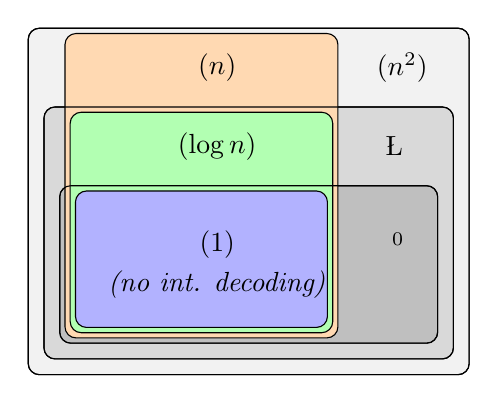
\begin{tikzpicture}
    \draw[rounded corners, fill=gray!10] (-2.4,-1.4) rectangle (3.2cm, 3cm);
    \draw[rounded corners, fill=gray!30] (-2.2,-1.2) rectangle (3.0cm, 2cm);
    \draw[rounded corners, fill=gray!50] (-2,-1) rectangle (2.8cm, 1cm);

    \draw[rounded corners, fill=orange!30] (-1.933,-0.933) rectangle (1.533cm, 2.933cm);
    \node at (0,2.5) {$\CoT(n)$};
    \draw[rounded corners, fill=green!30] (-1.867,-0.867) rectangle (1.467cm, 1.933cm);
    \node at (0,1.5) {$\CoT(\log n)$};
    \draw[rounded corners, fill=blue!30] (-1.8,-0.8) rectangle (1.4cm, 0.933cm);
    \node at (0,0.25) {$\CoT(1)$};
    \node at (0,-0.25) {\textit{(no int. decoding)}};

    \draw[rounded corners] (-2.4,-1.4) rectangle (3.2cm, 3cm);
    \draw[rounded corners] (-2.2,-1.2) rectangle (3.0cm, 2cm);
    \draw[rounded corners] (-2,-1) rectangle (2.8cm, 1cm);

    \node at (2.35,2.5) {$\tildeTIME(n^2)$};
    \node at (2.25, 1.5) {$\L$};
    \node at (2.3,0.25) {$\TC^0$};
    \end{tikzpicture}
    \quad\quad
    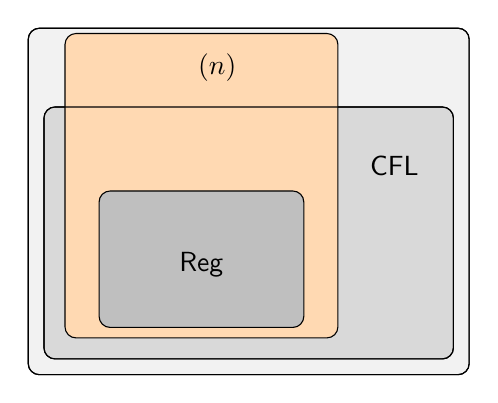
\begin{tikzpicture}
    \draw[rounded corners, fill=gray!10] (-2.4,-1.4) rectangle (3.2cm, 3cm);
    \draw[rounded corners, fill=gray!30] (-2.2,-1.2) rectangle (3.0cm, 2cm);

    \draw[rounded corners, fill=orange!30] (-1.933,-0.933) rectangle (1.533cm, 2.933cm);
    \node at (0,2.5) {$\CoT(n)$};

    \draw[rounded corners] (-2.4,-1.4) rectangle (3.2cm, 3cm);
    \draw[rounded corners] (-2.2,-1.2) rectangle (3.0cm, 2cm);
    \draw[rounded corners, fill=gray!50] (-1.5,-0.8) rectangle (1.1cm, 0.933cm);

    \node at (2.3,2.5) {$\CSL$};
    \node at (2.25, 1.25) {$\mathsf{CFL}$};
    \node at (-0.2,0) {$\mathsf{Reg}$};
    \end{tikzpicture}

    } % END resizebox
    
    \caption{
    Summary of results: transformers with intermediate generation against various classes of formal languages. A logarithmic number of chain-of-thought steps remains in log-space ($\mathsf L$). A linear number of steps adds more power, enabling recognizing all regular languages ($\mathsf{Reg}$), but is contained within context-sensitive languages ($\CSL$).
    We assume context-free languages ($\mathsf{CFL}$) require $\tilde \omega(n^2)$ time to recognize.
    Some regions with area in the plot are not known to be non-empty.
    }
    \label{fig:hierarchy}
\end{figure}


%%%%%%%%%%%%%%%%%%%%%%
\section{Results: The Power of Transformers with Intermediate Decoding}

% \citet{merrill2023parallelism} establish that uniform $\TC^0$ is an upper bound on the problems transformers can solve without generating intermediate tokens before answering, i.e., without a chain of thought. Informally, problems inside $\TC^0$ are efficiently parallelizable, while problems outside are inherently sequential. In this paper, we derive similar upper and lower bounds on the transformers \emph{with} a chain of thought, answering the question of by how much chain of thought extends transformers' reasoning power.

We next discuss our findings in more detail, both on the capabilities and the limits of transformer decoders with intermediate generation. Due to limited space, we defer all formal definitions, theorem statements, and proofs to the appendix, focusing here instead on the key results and one novel technical tool (namely, \emph{layer-norm hash}) used in our proofs. The formal models of transformer decoders and of multitape Turing machines underlying our results are discussed in \Cref{sec:prelim}, lower bounds proved in \Cref{sec:lower-bounds}, and upper bounds proved in \Cref{sec:upper-bounds}.

Let $\TIME(t(n))$ be the class of languages $L$ for which there exists a Turing machine that runs in time $\O(t(n))$ and accepts $L$.\footnote{As we will define later in the appendix, this is a non-random-access multitape Turing machine.} Let $\tildeTIME(t(n))$ be the class of problems in $\TIME(t(n) \log^k n)$ for some $k$, which is meaningful for $t(n) \geq n$.
Let $\SPACE(s(n))$ be the class of languages $L$ for which there exists a Turing machine with tape size bounded by $\O(s(n))$ that accepts $L$.
We show the following relationship between transformers with $t(n)$ steps and standard time/space complexity classes:
% \begin{equation} \label{eq:general}
%     \TIME(t(n)) \, \subseteq \, \CoT(t(n))
%     % \subseteq
%     \begin{array}{ll}
%         \subseteq \SPACE(t(n) + \log n) & \ \ \ \ \text{(Theorem~\ref{thm:space-ub})} \\
%         \subseteq \tildeTIME(t(n)^2 + n^2) & \ \ \ \ \text{(Theorem~\ref{thm:naive-upper-bound})}
%     \end{array} .
% \end{equation}=
\begin{align}
    \label{eq:lb}
    \TIME(t(n)) & \subseteq \, \CoT(t(n)) & & \text{(\Cref{cor:lower-bound})} \\
    \nonumber \ \\
    \label{eq:space-ub}
    \CoT(t(n)) & \subseteq \, \SPACE(t(n) + \log n) & & \text{(\Cref{thm:space-ub})} \\
    \label{eq:time-ub}
    \CoT(t(n)) & \subseteq \, \tildeTIME(t(n)^2 + n^2) & & \text{(\Cref{thm:naive-upper-bound})}
\end{align}
Both our time lower bound and space upper bound are fairly tight: improving either by a factor larger than $\log t(n)$ would result in a fundamental complexity theory advance \citep{Hopcroft1977OnTV}.

% \will{Could also use DTISP(t(n),s(n)) notation}
% See: https://complexityzoo.net/Complexity_Zoo:D#:~:text=DTISP(t(n)%2Cs(n))%3A,poly%2Cpolylog)

\paragraph{Capabilities of Transformers with CoT.} \Cref{eq:lb} implies that transformer decoders with $\Theta(n)$ steps can simulate real-time models of computation like automata or counter machines \citep{merrill2021linguistic}. Under standard assumptions in complexity theory, transformers with no decoding steps \emph{cannot} simulate all automata \citep{merrill2023parallelism,merrill23icgi,liu2023transformers}. Thus, a linear number of decoding steps makes transformers strictly more powerful. Similarly, \Cref{eq:lb} implies transformers with a \emph{quadratic} number of steps can express a linear-time algorithm (for a random access Turing machine) to solve directed graph connectivity \citep{wigderson1992complexity}, again a problem known to be beyond standard transformers.
% \will{CVP?} \ashish{would be good, but postpone until we are sure?} \will{sounds good}
With \emph{polynomial} decoding steps, transformers can solve linear equalities, Horn-clause satisfiability, and universal context-free recognition, all of which are $\P$-complete and thus inexpressible by standard transformers \citep{merrill2023parallelism}.
% or Horn satisfiability \ashish{cite?}, other problems that transformers with no decoding cannot solve. \will{requires independent construction}

Our proof shows that transformer decoders can simulate $t$ Turing machine steps with $t$ intermediate steps. Similar prior results have assumed external memory \citep{schuurmans2023memory} or an encoder-decoder model with nonstandard-positional decodings \citep{perez2021attention}. Our construction adapts these ideas to work for a decoder-only model \emph{without} external memory or extra positional encodings.\footnote{Our construction (\Cref{thm:lower-bound}) can be easily modified to work with an encoder-decoder model as well.}
% \citet{schuurmans2023memory} showed how a transformer language model could simulate a Turing machine in real time using external memory, but we show it can be done \emph{without external memory}. \citet{perez2021attention} showed how to simulate a Turing machine in real time using an encoder-decoder transformer with nonstandard positional encodings. Our construction adapts their idea to decoder-only models and, moreover, does not need to assume nonstandard positional encodings.


\paragraph{Limitations of Transformers with CoT.}
\Cref{eq:space-ub,eq:time-ub} establish two upper bounds on transformer decoders with $t(n)$ intermediate steps that depend on both $t(n)$ and $n$. We turn to the implications of this general result in different regimes for $t(n)$:

\begin{compactenum}
    \item \textbf{Log Steps}: Transformer decoders with $\O(\log n)$ intermediate steps can only recognize languages in $\L = \SPACE(\log n)$.
    % In comparison, transformers with no intermediate generation are in $\TC^0$, a subset of $\L$ \citep{merrill2023parallelism}. While the $\L$ upper bound is slightly weakened, it has many of the same implications as the $\TC^0$ upper bound.
    This implies that transformers with $\O(\log n)$ intermediate steps cannot solve $\NL$- or $\P$-complete problems$^{\ref{footnote:no-collapse-to-L}}$ like directed graph connectivity, just like transformers with no intermediate decoding \citep{merrill2023parallelism}.
    
    \item \textbf{Linear Steps}: Transformer decoders with $\O(n)$ intermediate steps can only recognize languages that are in both $\tildeTIME(n^2)$ and $\SPACE(n)$. Since $\SPACE(n)$ falls within the context-sensitive languages \citep{kuroda1964classes}, transformers with linear steps can recognize at most context-sensitive languages. Alongside our lower bound, this shows transformer decoders with $\Theta(n)$ steps fall somewhere between regular and context-sensitive languages in the Chomsky hierarchy. Further, transformers with $\O(n)$ steps cannot recognize all context-free languages unless context-free languages can be parsed in soft quadratic time.\footnote{The best known algorithms for context-free recognition run in time $\O(n^\omega)$, where $\omega$ is the matrix multiplication constant \citep{valiant1975general}; best lower bounds for context-free parsing are sub-quadratic \citep{lee2002fast}.}
    
    \item \textbf{Polynomial Steps}: If $t(n) = \O(n^c)$ for some $c$, we get an upper bound of $\P = \bigcup_{c=1}^\infty \TIME(n^c)$. Combined with our lower bound, this shows that transformer decoders with a polynomial number of steps recognize \emph{exactly} the class $\P$. Thus, a polynomial number of steps turns transformers into strong reasoners, though running a polynomial number of forward passes with a large transformer is likely intractable in practice.
\end{compactenum}

Together, these results show that intermediate generation like chain of thought or scratchpad can add reasoning power to transformers and that the number of steps matters as a computational resource akin to time or space. Some of the limitations identified in prior work \cite[][etc.]{merrill2023parallelism,chiang2023tighter} can be overcome with a linear or quadratic number of steps, and a polynomial number of steps covers all problems in $\P$. On the other hand, we have not identified any concrete reasoning problem where a logarithmic number of steps would help. These results provide a unified understanding of the power of transformer decoders across decoding lengths and problems.


\subsection{The Layer-Norm Hash}

The key idea behind our more general lower bound construction is the \textbf{layer-norm hash} (discussed in detail in \Cref{sec:lnorm-hash}): a simple module for effectively storing memory in decoder-only transformers.
% . Uniform attention is often useful for counting in algorithmic constructions for transformer encoders \citep{weiss2021thinking}, but causal attention masking makes this difficult in decoders because the denominator changes between tokens, obscuring the count value. The layer-norm hash fixes this problem by allowing us to easily compare counts computed via uniform attention \emph{independent of the denominator}.
We believe the layer-norm hash could be broadly useful for building algorithms in transformers.
For example, \citet{yao2021self} used a related idea to construct transformers that recognize bounded-depth Dyck languages, although in a more ad hoc way.

The layer-norm hash is a mechanism that enables retrieval across different columns in the transformer based on query-key matching of numerical values.
Exact-match retrieval is trivial when the query $q_i$ and keys $k_1, \ldots k_i$ are items in a finite set: just one-hot encode $q_i$ and $k_j$ and the inner product will be maximized when $q_i$ and $k_j$ match.
This, however, does not work when the keys and values are counts produced by uniform attention, which many transformer algorithms use \citep{weiss2021thinking}.
In this case, the key is a fraction $q_i/i$ and the queries are fractions $k_j/j$ with \emph{diferent} denominators.

The layer-norm hash helps by representing $q_i/i$ and $k_j/j$ such that hard attention retrieves the value $j$ where $q_i = k_j$. The idea is to use layer-norm to project $q_i$ and $k_j$ to vectors $\phi_{q_i}$ and $\phi_{k_i}$ on the unit sphere satisfying this property.
% where $\mathbf \phi_{q_i}^\top \cdot \phi_{k_j} = 0$ if and only if $q = k$.
Let $\lnorm(\mathbf x)  = \frac{\mathbf x'}{\norm{\mathbf x'}}$, where $\mathbf x' = \mathbf x - \bar x$. Then, the layer-norm hash of $x \in \mathbb R$ at position $i \in \mathbb N$ is a unit vector in $\mathbb R^4$ defined as:
% The layer-norm hash is a useful function computable by a transformer that enables comparing absolute counts between different columns in the transformer. Concretely, imagine $q/n$ is a fraction computed by taking uniform attention over $n$ previous positions. For any $q \in \mathbb R$, $n \in \mathbb N$, the layer-norm hash is a vector representation of this scalar:
    \begin{equation*}
        \hash(x/i, 1/i) = \lnorm \left( \frac{x}{i}, \frac{1}{i}, -\frac{x}{i}, -\frac{1}{i} \right) .
    \end{equation*}
A key feature of this representation is that it is invariant w.r.t.\ $i$ in the sense that $\hash(x/i, 1/i) \triangleq \hash_x$ is only a function of $x$, independent of $i$.
Further, the inner products of these representations of two scalars $q, k$ is maximized to $1$ if and only if $q = k$.
% \begin{restatable}{lemma}{lnormhash} \label{lem:lnorm-hash}
%     For $q, k \in \mathbb{R}, i, j \in \mathbb N$, $\hash(q/i, 1/i) \cdot \hash(k/j, 1/j)$ is maximized exactly when $q = k$.
% \end{restatable}
We can thus look up key $q_i/i$ in a sequence of keys $k_1/1, \ldots, k_i/i$ by attending with query $\hash(q_i/i, 1/i) = \hash_{q_i}$ at position $i$ and key $\hash(k_j/j, 1/j) = \hash_{k_j}$ at each position $j$.
This retrieves the value at $j$ such that $q_i = k_j$.
% The layer-norm hash can also be used to directly compare two values $q_i, k_j$ without removing the denominator by computing $\hash(q_i, 1)$ and $\hash(k_j, 1)$.



\section{Discussion}

We have shown that intermediate decoding steps extend the formal power of transformers well beyond previously known upper bounds, such as $\TC^0$ circuits and $\FOM$ logic, on transformers without intermediate decoding. Further, the amount of additional power is closely related to the number of decoding steps. In particular, transformers with a linear number of decoding steps have the capacity to recognize regular languages, but cannot recognize languages beyond context-sensitive. With a log number of decoding steps, such transformers can only recognize languages in $\L$, which is a complexity class relatively close to $\TC^0$. Thus, it appears that a linear number of intermediate decoding steps may be required to overcome the limitations of transformers on many sequential reasoning problems of interest.
In future work, it may be possible to derive a strict separation between transformers with a log and a linear number of decoding steps and show that certain problems that currently have a quadratic bound can in fact be solved with a roughly linear number of steps.

% Similarly, it would be interesting to consider intermediate values for $t(n)$ such as $\sqrt{n}$ or $n / \log n$.

Here we have focused on lower and upper bounds on expressive power, rather than analyzing learnability. 
Whereas our upper bounds directly reveal limitations on what transformers with intermediate generation can learn, one caveat is that our lower bounds \emph{do not} directly imply transformers can learn to use intermediate steps effectively.
% In particular, since language models cannot condition on their previous output during training, we hypothesize that it may be difficult for transformer LMs to learn how to reliably reason with generated tokens if a chain of thought is added post hoc.
It would be interesting to formally investigate transformers with CoT from a learning-theoretic lens, possibly along the lines of \citet{malach2023autoregressive}, and how different kinds of fine-tuning, such as reinforcement learning, might improve a model's ability to use the power of its chain of thought.

% Will: would be interesting to extend to random-access machines.
% \ashish{Two people have mentioned one angle that we could potentially list as an important open problem: characterize the effect of model size on transformer CoT ability, e.g., explain why CoT seems to "emerge" only for large enough models. I'm not sure what we can say here though, as our TM simulation seems fairly straightforward and simplistic in terms of the computation at each step.}

% Acknowledgements should only appear in the accepted version.
% \section*{Acknowledgements}
% Jason Wei, Ofir Press, Abulhair Saparov, Avi Wigderson
% NYU requirement: NSF Award 1922658

% \subsubsection*{Author Contributions}
% If you'd like to, you may include  a section for author contributions as is done
% in many journals. This is optional and at the discretion of the authors.

% \subsubsection*{Acknowledgments}
% Use unnumbered third level headings for the acknowledgments. All
% acknowledgments, including those to funding agencies, go at the end of the paper.

\bibliography{references}
\bibliographystyle{iclr2024_conference}

\appendix
\input{neurips-workshop/appendix-new}
\input{neurips-workshop/appendix-orig}

\end{document}